\documentclass[sigconf,nonacm,screen]{acmart}

% ---------------------------------------------------------------------------------------------
% Project report. Build: latexmk -pdf report.tex   (figures are produced by ../code/figures/*.py)
% ---------------------------------------------------------------------------------------------
\settopmatter{printacmref=false,printfolios=true}
\renewcommand\footnotetextcopyrightpermission[1]{}
\pagestyle{plain}

\usepackage{graphicx}
\usepackage{booktabs}
\usepackage{enumitem}
\graphicspath{{figures/}}
\setlist{nosep,leftmargin=*}

\newcommand{\R}{\mathbb{R}}
\newcommand{\conv}{\operatorname{conv}}
\newcommand{\LN}{\operatorname{LN}}
\newcommand{\msum}{\oplus}
\newcommand{\bigmsum}{\bigoplus}
\newcommand{\simplex}{\Delta}
\newcommand{\one}{\mathbf{1}}
\newcommand{\X}{\mathcal{X}}
\newcommand{\cP}{\mathcal{P}}
\newcommand{\cT}{\mathcal{T}}
\newcommand{\cS}{\mathcal{S}}
\newcommand{\cE}{\mathcal{E}}
\newcommand{\rank}{\operatorname{rank}}
\newcommand{\softmax}{\operatorname{softmax}}
\newcommand{\pending}[1]{\textcolor{red}{[#1]}}

\title{Box or Simplex? A Critical Study of the Minkowski Representation Hypothesis}
\subtitle{Project report on ``Into the Rabbit Hull'' (Fel, Wang et al., ICLR 2026)}

\author{Omar Besbes}
\affiliation{%
  \institution{Master MVA, ENS Paris-Saclay}
  \country{France}}

\begin{abstract}
\pending{abstract: written last}
\end{abstract}

\begin{document}

\begin{teaserfigure}
  \centering
  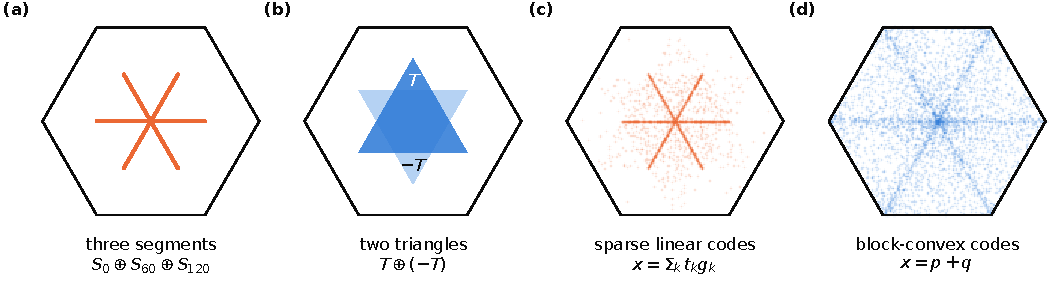
\includegraphics[width=\textwidth]{fig_hexagon}
  \caption{\pending{teaser caption}}
  \Description{Four panels showing a regular hexagon written as a sum of three segments and as a sum of two triangles, and two point clouds with this support.}
  \label{fig:hexagon}
\end{teaserfigure}

\maketitle

% =============================================================================================
\section{Introduction}
\label{sec:intro}

Vision transformers trained without labels, such as DINOv2~\cite{oquab2024dinov2}, produce features that
solve classification, segmentation and depth estimation with a single linear layer. What these features
encode, and how, is the question of \emph{interpretability}. The dominant working assumption is the
\emph{linear representation hypothesis} (LRH)~\cite{elhage2022superposition,park2024linear}: an activation
is a sparse combination of many more directions than there are dimensions. It turns interpretability into
a dictionary-learning problem, solved in practice by sparse autoencoders
(SAEs)~\cite{bricken2023monosemanticity,cunningham2024sparse}.

\citet{fel2026rabbit} take this assumption seriously, at scale, on DINOv2. They train a dictionary of
$32{,}000$ atoms and use it in three ways. First, they ask which atoms each downstream task relies on, and
find specialised families, among them ``Elsewhere'' concepts that fire everywhere except on the object
they depend on. Second, they study the statistics and geometry of the dictionary and report features
that a sparse, nearly orthogonal code does not predict: dense positional atoms, antipodal pairs,
clustered and anisotropic atoms, and token clouds that look smooth within an image. Third, they propose
an alternative, the \emph{Minkowski representation hypothesis} (MRH): a token is a sum of a few convex
combinations of ``archetypes'', so that the set of activations is a Minkowski sum of polytopes. They
support it with an argument on attention, with three empirical signatures, and draw consequences for
steering and for the identifiability of concepts.

The third part is the boldest, and the authors are careful to call it a working hypothesis. This report
examines it. We ask three questions that a hypothesis about geometry must answer: what exactly does it
assert that its predecessor does not, what do the arguments given for it establish, and what observation
could contradict it? Following the philosophy of the class, we answer with definitions, short proofs and
small examples rather than with a new benchmark; the experiments on DINOv2 itself are deliberately small
and serve as checks. Our contributions are the following.

\begin{itemize}
  \item \textbf{Two nested hypotheses (\S\ref{sec:nested}).} LRH with bounded codes is the special case of
  MRH in which every polytope is a segment. The two hypotheses differ only in how the codes of a group
  are coupled, by a box or by a simplex, and the support of the activations cannot tell them apart: the
  regular hexagon is at once a sum of three segments and a sum of two triangles
  (Figure~\ref{fig:hexagon}).
  \item \textbf{Limits of the architectural argument (\S\ref{sec:attention}).} That attention outputs sums
  of convex combinations is true for any weights and any input, of vectors that change with the image.
  We show that the final layer normalisation places every token on an ellipsoid that contains no
  segment, so that no non-trivial Minkowski sum describes the normalised activations exactly.
  \item \textbf{The three signatures under null models (\S\ref{sec:diagnostics}).} \pending{one sentence per
  finding once the experiments are final}
  \item \textbf{Identifiability (\S\ref{sec:identifiability}).} We repair the proof of the
  non-identifiability result and argue that it does not single out MRH: it concerns supports, it applies
  word for word to linear codes, and it ignores the two ingredients, sparsity and the law of the codes,
  on which the identifiability of dictionaries has always rested.
\end{itemize}

% =============================================================================================
\section{Context: concepts as sparse directions}
\label{sec:context}

\paragraph{Model.} DINOv2~\cite{oquab2024dinov2} is a vision transformer~\cite{dosovitskiy2021image}
trained by self-distillation~\cite{caron2021emerging,zhou2022ibot}. The model studied in the paper, ViT-B/14
with registers~\cite{darcet2024registers}, maps a $224\times224$ image to $t=261$ tokens of dimension
$d=768$: one class token, four registers and $16\times16$ patch tokens. Each of its 12 blocks adds to
every token the output of a multi-head attention layer (12 heads of dimension 64) and of an MLP, each
preceded by a layer normalisation~\cite{ba2016layer}; a last normalisation is applied to the output.

\paragraph{The linear representation hypothesis.} A representation $x\in\R^d$ satisfies the LRH if
\begin{equation}
  x=\sum_{j=1}^{c} z_j d_j ,\qquad \|z\|_0\le k\ll c,\qquad c\gg d,
  \label{eq:lrh}
\end{equation}
for a dictionary of unit vectors $d_1,\dots,d_c$ with small mutual coherence $\max_{i\neq j}|\langle
d_i,d_j\rangle|$. Sparsity makes room for more features than dimensions
(\emph{superposition}~\cite{elhage2022superposition}), and low coherence limits their interference; the
optimal arrangements are Grassmannian frames~\cite{strohmer2003grassmannian}. Recovering $(d_j)$ and $z$
from activations is sparse dictionary learning~\cite{olshausen1996emergence}. The paper places the classical
concept-extraction methods in one family, $\min\|A-ZD\|_F^2$ under a constraint: $k$-means (one-hot codes),
PCA (orthogonal atoms), NMF (non-negative factors), archetypal analysis~\cite{cutler1994archetypal} (codes
in a simplex, atoms in the convex hull of the data) and SAEs (codes computed by an encoder, with a
sparsity projection). As \citet{hindupur2025projecting} stress, each member of the family presupposes a
geometry of the concepts and can only find concepts of that shape.

\paragraph{The dictionary.} Plain SAEs are unstable across training runs~\cite{paulo2025sparse}. The paper
uses an archetypal SAE~\cite{fel2025archetypal}, whose atoms are constrained to the convex hull of
$128{,}000$ centroids of the data, with non-negative codes and $k=8$ active atoms per token on average
(BatchTopK~\cite{bussmann2024batchtopk}). Trained on the tokens of 1.4 million ImageNet images, it explains
more than 88\% of their variance.

\paragraph{What tasks use.} For a linear probe $y=Wx$, the contribution of atom $j$ to output $o$ is
$\mathbb{E}[z_j]\,\langle w_o,d_j\rangle$, which is exact because everything is
linear~\cite{fel2023holistic}. Ranking atoms by this score, the paper finds that classification draws on a
broad set of atoms, while segmentation and depth use compact families: border detectors, and three groups
of monocular depth cues (perspective, shading, changes of local frequency). The most original finding is
the ``Elsewhere'' concept: an atom that fires on the tokens \emph{not} covered by an object and only when
the object is present, as a masking analysis~\cite{petsiuk2018rise} confirms. Where a concept fires is
therefore not what it is about, which is a warning for every heat map. A further family lives on the
register tokens only and encodes global properties of the scene (blur, illumination, lens distortion).

\paragraph{Cracks in the linear picture.} The second part of the paper measures the dictionary against the
LRH. Three atoms fire on roughly a quarter of all tokens each and encode the position of the token (left,
right, bottom): they are dense~\cite{sun2025dense}, not sparse. The inner products between atoms have much
heavier tails than those of random vectors, let alone of a Grassmannian frame, and the singular values
of the dictionary decay sharply: atoms cluster, and the clusters follow the tasks. Some pairs are
antipodal ($d_i\approx-d_j$) and encode opposite ends of one axis. Finally the tokens of one image, coloured
by their first principal components, form smooth maps that survive the removal of positional information,
whose own geometry collapses from a high-rank code in the early layers to a two-dimensional sheet in the
last ones.

\paragraph{Other departures from linearity.} The paper is one of several recent proposals that replace
directions by richer objects: irreducible multi-dimensional features such as circles~\cite{engels2025not},
polytopes for categorical variables~\cite{park2025geometry}, the linear regions of the
network~\cite{black2022polytope}, or local low-dimensional regions fitted by mixtures of factor
analysers~\cite{shafran2026directions}. Its cognitive motivation is the theory of conceptual
spaces~\cite{gardenfors2000conceptual}, in which a concept is a convex region around a prototype.

% =============================================================================================
\section{The Minkowski representation hypothesis}
\label{sec:mrh}

\paragraph{Statement.} Let $a_1,\dots,a_c\in\R^d$ be \emph{archetypes}, partitioned into $m$ \emph{tiles}
$\cT_1,\dots,\cT_m$, and let $\cP_i=\conv\{a_j:\ j\in\cT_i\}$. Writing $A\msum B=\{a+b:\ a\in A,\ b\in B\}$
for the Minkowski sum, the set $\X$ of activations of a layer satisfies the MRH if
\begin{equation}
  \text{(i)}\ \ \X=\bigmsum_{i=1}^{m}\cP_i ,\qquad
  \text{(ii)}\ \ x=\sum_{i\in S}\ \sum_{j\in\cT_i} z_j a_j,\quad z_{\cT_i}\in\simplex,\quad |S|\ll m,
  \label{eq:mrh}
\end{equation}
where $\simplex$ is the probability simplex: every activation is a sum of a few points, one in each active
polytope. A token showing a rabbit would be the sum of a point of an ``animal'' polytope near its rabbit
archetype, of a point of a ``position'' polytope, and so on. A concept is then a point or a region, not a
direction, and evidence for it is proximity to an archetype, not the size of an inner product.

\paragraph{Why attention would produce it.} A head with attention weights $\alpha\in\simplex^{t}$ and
value vectors $v_1,\dots,v_t$ outputs $\sum_j\alpha_j v_j\in\conv\{v_j\}$, and a layer with $H$ heads
outputs
\begin{equation}
  y=\sum_{h=1}^{H}W_O^{(h)}\sum_{j=1}^{t}\alpha_{h,j}\,v_{h,j}\ \in\ \bigmsum_{h=1}^{H}W_O^{(h)}\conv\{v_{h,j}\}_j ,
  \label{eq:mha}
\end{equation}
because linear maps send hulls to hulls. The paper adds that the inclusion in~\eqref{eq:mha} is an equality
if the logits of each head can reach every vector of $\R^t$ up to a constant, that affine maps preserve
convex codes, and that sharp attention concentrates the output on vertices or faces.

\paragraph{Evidence.} Three observations on last-layer tokens are offered as ``compatible evidence, not
proof''. (E1)~Along the straight segment between two tokens, the distance to the nearest token grows to a
peak at the midpoint, whereas along a shortest path in the $k$-nearest-neighbour graph it stays small.
(E2)~Archetypal analysis fitted on the 256 tokens of one image reconstructs them better than the SAE as
soon as it has ten archetypes. (E3)~The co-activation matrix $A^\top A$ of the codes $A$ of an archetypal
analysis is block-diagonal after clustering.

\paragraph{Consequences.} (I1)~Concepts are landmarks and regions. (I2)~Steering towards an archetype
saturates when it is reached, which would explain why steering along SAE directions stops working at
large amplitudes~\cite{templeton2024scaling}. (I3)~A Minkowski sum does not determine its summands, so
concepts cannot be recovered from the activations of one layer; one should use the attention weights and
the earlier layers.

% =============================================================================================
\section{Analysis}
\label{sec:analysis}

\subsection{Two nested hypotheses: box or simplex}
\label{sec:nested}

Definition~\eqref{eq:mrh} needs one repair before it can be compared with~\eqref{eq:lrh}. A Minkowski sum
of convex sets is convex, and a point of $\bigmsum_{i=1}^m\cP_i$ receives a contribution from every tile,
whereas (ii) uses a few tiles only. The two items agree only if inactive tiles contribute a fixed point,
and the set that the text describes (``a union over attention patterns'') is
\begin{equation}
  \X=\bigcup_{S\in\cS}\ \bigmsum_{i\in S}\cP_i ,
  \label{eq:union}
\end{equation}
a union of polytopes indexed by the admissible active sets. This is the exact counterpart of sparse
coding, whose activations fill a union of low-dimensional cones. The parallel can be made precise.

\begin{proposition}[Nested hypotheses]
\label{prop:nested}
(a) Let $x=\sum_{j\in S}z_jd_j$ with $|S|\le k$ and $0\le z_j\le M$. Then $x$ satisfies~\eqref{eq:mrh}(ii)
with the same active set and the two-point tiles $\cT_j=\{0,\,Md_j\}$.
(b) Conversely, a code satisfying~\eqref{eq:mrh}(ii) is a non-negative linear code over the dictionary of
archetypes, with at most $\sum_{i\in S}|\cT_i|$ non-zero entries, subject to the $|S|$ equalities
$\sum_{j\in\cT_i}z_j=1$.
\end{proposition}
\begin{proof}
(a) $z_jd_j=(1-z_j/M)\,0+(z_j/M)\,Md_j$ is a convex combination of the two archetypes of $\cT_j$.
(b) is a rewriting of~\eqref{eq:mrh}(ii).
\end{proof}

With signed codes, replace $\cT_j$ by $\{-Md_j,Md_j\}$. Since activations are bounded, (a) says that
\emph{every} representation satisfying the LRH satisfies the MRH with segments as tiles: its set of
activations is a union of zonotopes. Conversely a tile with two archetypes $\{a,b\}$ contributes
$a+\lambda(b-a)$, a bounded linear feature along $b-a$ with an offset. The hypotheses therefore part
ways only at tiles with three archetypes or more, and there the difference is the feasible set of the
codes: for a tile $\{a,b,c\}$, the coordinates $(\lambda_b,\lambda_c)$ of $a+\lambda_b(b-a)+\lambda_c(c-a)$
range over the triangle $\lambda_b+\lambda_c\le1$ under MRH, and over a square under LRH, where the two
features are free to be large together. \emph{Inside a tile, features share a unit budget; across tiles
they do not.} A tile is thus an irreducible multi-dimensional feature in the sense of
\citet{engels2025not}, and MRH is LRH plus a statement of mutual exclusion inside groups of atoms: a
categorical variable relaxed to its simplex.

\paragraph{The hexagon.} The budget is a property of the codes, not of the set they generate. Let
$g_1,g_2,g_3$ be unit vectors at angles $0^\circ,60^\circ,120^\circ$, let $S_k=[-g_k/2,\,g_k/2]$, and let
$T$ be an equilateral triangle with unit sides. Then the regular hexagon $H$ of unit circumradius satisfies
\begin{equation}
  H \;=\; S_1\msum S_2\msum S_3 \;=\; T\msum(-T).
  \label{eq:hexagon}
\end{equation}
The first expression is a linear code with three bounded features in superposition in the plane; the
second is a block-convex code with two ternary tiles (Figure~\ref{fig:hexagon}a--b). No property of the set
$H$ can decide between them. What differs is the law of the points: sparse independent codes put most of
their mass on the three lines spanned by the $g_k$, whereas codes concentrated near the archetypes put it
near the nine sums of vertices (Figure~\ref{fig:hexagon}c--d). The lesson for what follows is that a test
of MRH against LRH must bear on the joint statistics of the codes; a test that only asks where
activations lie cannot succeed.

\subsection{What the attention argument shows}
\label{sec:attention}

Equation~\eqref{eq:mha} is correct, and it is a statement about softmax, not about DINOv2. Four
observations delimit what it implies for the representation.

\paragraph{The polytopes are rebuilt for every image.} The values of head $h$ are $v_{h,j}=W_V^{(h)}\LN(x_j)$,
where $x_1,\dots,x_t$ are the tokens of the current image at the previous layer. The polytope
$\conv\{v_{h,j}\}_j$ is therefore a function of the image: \eqref{eq:mha} says that the update of a token
is a mixture of the other tokens of its image, seen through $H$ linear maps. It holds verbatim for a
network with random weights and for an input of pure noise, so it cannot by itself explain anything that
DINOv2 has learned. The MRH is a stronger claim, that of a \emph{fixed} dictionary of archetypes shared
by all images, and that claim would require the values of all images to concentrate near a common finite
set, which \eqref{eq:mha} does not address.

\paragraph{Equality is out of reach.} The logits of a head are $Kq$, where the rows of
$K\in\R^{t\times d_k}$ are the keys and $q\in\R^{d_k}$ is the query. They span a space of dimension at most
$d_k=64$, while the condition for equality in~\eqref{eq:mha} asks for $\rank K+1\ge t=261$. In addition
the query of a token is tied to that token, so an image realises exactly $t$ points of each polytope.
\pending{R4: measured rank; attention entropy / effective support}

\paragraph{An update is not a token.} The representation that is analysed is the residual stream,
$x^{(L)}=x^{(0)}+\sum_{\ell}a^{(\ell)}+\sum_\ell m^{(\ell)}$, where $a^{(\ell)}$ are attention updates and
$m^{(\ell)}$ are outputs of MLPs, to which~\eqref{eq:mha} does not apply. \pending{R4: fractions f_attn,
f_mlp of the final token}

\paragraph{The last normalisation leaves no room for a polytope.} The standard features of DINOv2, and
the activations that the paper itself describes as lying on an ``ellipsoidal geometry'' (its footnote~5),
are read after a final layer normalisation $\LN(x)=\gamma\odot\frac{x-\mu(x)\one}{\sigma(x)}+\beta$, with
$\mu$ and $\sigma$ the mean and standard deviation of the coordinates of $x$. This map is not affine, and
its range is thin~\cite{brody2023expressivity}.

\begin{proposition}[No segment after layer normalisation]
\label{prop:ellipsoid}
Assume $\gamma_k\neq0$ for all $k$ and neglect the stabilising constant in $\sigma$. Then the range of
$\LN$ is contained in an ellipsoid $\cE$ of dimension $d-2$, and:
(a) for two distinct outputs $y\neq y'$, no point $(1-s)y+sy'$ with $0<s<1$ belongs to $\cE$;
(b) if a set $\X\subseteq\cE$ is a Minkowski sum $\cP_1\msum\dots\msum\cP_m$, then every $\cP_i$ is a
single point.
\end{proposition}
\begin{proof}
The vector $u=(x-\mu(x)\one)/\sigma(x)$ satisfies $\one^\top u=0$ and $\|u\|^2=d$: it lies on a sphere $\mathbb{S}$
of the hyperplane $\one^\perp$. The map $\Phi(u)=\gamma\odot u+\beta$ is affine and injective, and
$\cE=\Phi(\mathbb{S})$. (a) By strict convexity of the Euclidean norm, $\|(1-s)u+su'\|<\sqrt d$ for $u\ne u'$ in
$\mathbb{S}$, so the open segment between $u$ and $u'$ misses $\mathbb{S}$; its image by $\Phi$ is the open segment
between $y$ and $y'$, and it misses $\Phi(\mathbb{S})$ because $\Phi$ is injective. (b) If some $\cP_i$ contains
$p\neq p'$, choose $q_j\in\cP_j$ for $j\neq i$: then $\sum_{j\ne i}q_j+[p,p']\subseteq\X\subseteq\cE$ is a
segment inside $\cE$, which contradicts (a).
\end{proof}

Item (b) says that~\eqref{eq:mrh}(i), and its repaired form~\eqref{eq:union}, cannot hold exactly for
normalised tokens, whatever the archetypes: at best the MRH is a local approximation, valid at scales
where the ellipsoid is flat. Item (a) says that signature (E1) is automatic: a chord between two tokens
leaves the set of attainable activations as soon as it starts. The midpoint of a chord subtending an
angle $\theta$ on $\mathbb{S}$ lies at depth $(1-\cos\frac\theta2)\sqrt d$ below the sphere.
\pending{R1: measured angles and depths, within and across images; Figure}
The LRH is affected as well, since on $\cE$ a code cannot be doubled, but definition~\eqref{eq:lrh} is a
statement about each activation and survives, as does~\eqref{eq:mrh}(ii); only the set-level claim (i) is
excluded.

\subsection{Three signatures under null models}
\label{sec:diagnostics}
\pending{E1 chords: toy T1 + DINOv2 R2. E2 archetypal analysis: sandwich, toy T2 + R3. E3 co-activation: sum vs union, toy T3 + R5.}

\subsection{Identifiability}
\label{sec:identifiability}

\paragraph{The proof.} The paper derives (I3) from the additivity of support functions,
$h_{A\msum B}=h_A+h_B$ with $h_C(u)=\sup_{x\in C}\langle u,x\rangle$: decomposing $\X$ amounts to writing
$h_\X$ as a sum of sublinear functions. Its proof then picks ``any sublinear $s$ with $0\le s\le h_\X$''
and writes $h_\X=(h_\X-s)+s$. This step fails, because $h_\X-s$ need not be sublinear: it is so exactly
when the convex set with support function $s$ is a summand of $\X$. For a triangle $\X$ centred at the
origin and a short segment $Q\subset\X$, the function $s=h_Q$ satisfies $0\le s\le h_\X$, yet a triangle
has no summand other than its own homothets~\cite{schneider2014convex}. \pending{T4c: explicit u, v with
f(u+v) > f(u)+f(v)} The statement survives in a weaker form. Decompositions are never unique, for three
trivial reasons: summands can be translated in opposite directions, a summand can be split as
$\cP=\lambda\cP\msum(1-\lambda)\cP$, and summands can be regrouped. The rectangle that the paper cuts into
three segments is an instance of the second and third. Up to these operations, a polytope is a sum of
indecomposable ones~\cite{smilansky1987decomposability,schneider2014convex}, and this decomposition is not
unique either:~\eqref{eq:hexagon} is the classical example, segments and triangles being indecomposable.

\paragraph{What it does not show.} The corrected statement concerns the \emph{support} of the activations
when \emph{all} tiles are active. Under the same reading the LRH fares no better: the set
$\{\sum_jz_jd_j:\ z\in[0,M]^c\}$ generated by a dense linear code is a zonotope, and~\eqref{eq:hexagon}
shows that it does not determine its generators, nor even whether it comes from a linear code. Nobody
concludes from this that sparse dictionaries cannot be learned from one layer. Dictionaries are
identifiable because codes are sparse~\cite{donoho2003optimally,aharon2006uniqueness} and because their
coordinates are statistically independent and non-Gaussian~\cite{comon1994independent}; both properties
concern the law of the data on its support. The MRH has the same resources: its item (ii) is a sparsity
assumption, which turns the support into the union~\eqref{eq:union}, whose low-dimensional pieces
expose the individual polytopes; and the two clouds of Figure~\ref{fig:hexagon} (c--d), which share their
support, are told apart at a glance. Consequence (I3) is thus too strong as stated. The practical advice
of the paper stands on its own merits: attention weights are available, and they are the codes
of~\eqref{eq:mha}.

\subsection{A tile that can be observed: position}
\label{sec:position}
\pending{R6: additivity of the position code; zonotope reading.}

% =============================================================================================
\section{Discussion}
\label{sec:discussion}
\pending{what stands; what would count as evidence; limitations of this study.}

\bibliographystyle{ACM-Reference-Format}
\bibliography{refs}

\end{document}
